
\documentclass{article} % For LaTeX2e
\usepackage{style,times}
\usepackage{amsmath,amsfonts,bm,amssymb}
\usepackage{graphicx}

%%%%% customized by shuo begin


\DeclareMathOperator*{\argmax}{argmax}
% \usepackage[hidelinks]{hyperref}
\usepackage{hyperref}
\usepackage{url}
\usepackage{subcaption}
\usepackage{algorithm}
\usepackage{algorithmic}
\usepackage{amsthm}
\newtheorem{theorem}{Theorem}
\newtheorem{definition}{Definition}
\newtheorem{fact}{Fact}
\newtheorem{proposition}{Proposition}

\newcommand{\red}[1]{\textcolor{red}{#1}}
%%%% customized by shuo end

\title{A Brief Introduction to Dec-POMDP}

\author{Shuo Liu \\
Computer Science\\
Northeastern University\\
\texttt{shuo.liu2@northeastern.edu} \\
}

\iclrfinalcopy % Uncomment for camera-ready version, but NOT for submission.
\begin{document}


\maketitle
\vspace{-6mm}
\begin{abstract}
This article introduces Dec-POMDP, the computation, and planning methods.\footnote{This introduction is \textbf{heavily} based on \cite{DecPOMDPsurvey}.}
\end{abstract}

\section{Dec-POMDP}

\begin{definition}
    A Dec-POMDP is a tuple $\langle \mathbb{I}, \mathcal{S}, \{\mathbb{A}_i\}, T, R, \{\mathbb{O}_i\}, O, \mathcal{H}, \gamma\rangle$:
    \begin{itemize}
    \item $\mathbb{I}$ is a finite sets of agents, $|\mathbb{I}|=n$;
    \item $\mathcal{S}$ is a set of states with designated initial state distribution $b^0$;
    \item $\mathbb{A}_i$ is a set of actions for agent $i$ with $\mathbb{A}\doteq \times_i \mathbb{A}_i$ the set of joint actions;
    \item $T$ is the state transition probability function, $T$: $\mathcal{S} \times \mathbb{A} \times \mathcal{S} \rightarrow [0, 1]$, that specifies the probability of transitioning from state $s \in \mathcal{S}$ to $s' \in \mathcal{S}$ when the actions $\boldsymbol{a} \in \mathbb{A}$ are taken by agents (i.e., $T(s, \boldsymbol{a}, s')=P(s'|s, \textbf{a})$);
    \item $R$ is the joint reward function, where $R$: $\mathcal{S} \times \mathbb{A} \rightarrow \mathbb{R}$;
    \item $\mathbb{O}_i$ is a set of observations for each agent $i$, with $\mathbb{O}\doteq\times_i \mathbb{O}_i$ the set of joint observations;
    \item $O$ is an observation probability function, $O$: $\mathbb{A} \times \mathcal{S} \times \mathbb{O}$, that specifies the probability of seeing observation $\boldsymbol{o}' \in \mathbb{O}$ given the actions $\boldsymbol{a} \in \mathbb{A}$ are taken and state $s' \in \mathcal{S}$ is observed (i.e., $O(\boldsymbol{a}, s', \boldsymbol{o}')=P(\boldsymbol{o}'|\textbf{a},s')$);
    \item $\mathcal{H}$ is the horizon (the number of steps until termination);
    \item $\gamma$ is the discount factor for the return. 
\end{itemize}

A solution to a Dec-POMDP is a joint policy $\boldsymbol{\pi}:\mathbb{H}_i\to\mathbb{A}_i, \forall i \in \mathbb{I}$ over joint observation-action history $\boldsymbol{h}=\{\boldsymbol{a}^{0}, \boldsymbol{o}^{1}, \cdots \boldsymbol{o}^{\mathcal{H}-1}\}$, an optimal solution maximizes the expected return,
\[
\boldsymbol{\pi}^*=\argmax_{\boldsymbol{\pi}}\mathbb{E}\left[\textstyle\sum_{t=0}^{\mathcal{H}-1}R(\boldsymbol{h}, \boldsymbol{\pi}(\boldsymbol{h}))\middle|b^0\right].
\]
\end{definition}

In Dec-POMDP, the Bellman recursive formulation of the history V-function is,
\begin{equation}\label{eq:decpomdp-V}
\begin{aligned}
    V^{\boldsymbol{\pi}}(\boldsymbol{h}) &= \sum_{s} P(s|b^0, \boldsymbol{h})\left[R(s, \boldsymbol{\pi}(\boldsymbol{h}))+\gamma \sum_{s'}P(s'|s, \boldsymbol{\pi}(\boldsymbol{h})) \sum_{\boldsymbol{o}'}P(\boldsymbol{o}'|\boldsymbol{\pi}(\boldsymbol{h}), s') V^{\boldsymbol{\pi}}(\boldsymbol{h}') \right]\\
    &\equiv R(\boldsymbol{h}, \boldsymbol{\pi})+\gamma\sum_{\boldsymbol{o}'}P(\boldsymbol{o}'|\boldsymbol{h}, \boldsymbol{\pi}) V^{\boldsymbol{\pi}}(\boldsymbol{h}'),
\end{aligned}
\end{equation}
the Bellman recursive formulation of the \textbf{history-policy} Q-function is,\footnote{The definition of the value function is pretty flexible, which can be based on various aspects, such as the value of a state, a belief state, an observation, a state history, an observation history, an action (single-step policy), a policy (action history), observation-action history, and their combinations.}
\begin{equation}\label{eq:decpomdp-q}
\small
\begin{aligned}
    Q^{\boldsymbol{\pi}}(\boldsymbol{h}, \boldsymbol{\pi}) &= \sum_{s} P(s|b^0, \boldsymbol{h})\left[R(s, \boldsymbol{\pi}(\boldsymbol{h}))+\gamma\sum_{s'}P(s'|s, \boldsymbol{\pi}(\boldsymbol{h})) \sum_{\boldsymbol{o}'}P(\boldsymbol{o}'|\boldsymbol{\pi}(\boldsymbol{h}), s') Q^{\boldsymbol{\pi}}(\boldsymbol{h}', \boldsymbol{\pi}(\boldsymbol{h}')) \right]\\
    &\equiv R(\boldsymbol{h}, \boldsymbol{\pi})+\gamma\sum_{\boldsymbol{o}'}P(\boldsymbol{o}'|\boldsymbol{h}, \boldsymbol{\pi}) Q^{\boldsymbol{\pi}}(\boldsymbol{h}', \boldsymbol{\pi}) .
\end{aligned}
\end{equation}


\section{Subclasses}

\paragraph{Centralized Control}
MMDP is a fully observable version of Dec-POMDP, but it does not specify decentralized control. Dec-MDP assumes that the joint observations uniquely determine the state, while agents still act with local observations. Similarly, MPOMDP does not specify whether the control is decentralized, which could have a centralized policy $\mathbb{H}\to\mathbb{A}$.

\paragraph{Independent Variables}
A decentralized control model might be factorized with independent local variables, e.g., transition-independence (TI) $T(s, \boldsymbol{a}, s')=\Pi_{i=1}^{n} T(s_i, a_i, s_i')$ and reward-independence (RI) $R(s,\boldsymbol{\pi})=f_\text{mono}(\langle R(s_i, \pi_i)\rangle_{i=1}^{n})$. Network-distributed POMDP (ND-POMDP) represents the factored one with TI and block-RI, i.e., $R(s,\boldsymbol{\pi})=f_\text{mono}(\langle R(s_{i, \mathcal{N}(i)}, \pi_{i, \mathcal{N}(i)})\rangle_{i=1}^{n})$, where ${\mathcal{N}(i)}$ are the neighbors of $i$.

\paragraph{Complexity} The worst-case complexity of finite-horizon problems is: (by \cite{DecPOMDPsurvey})

\renewcommand{\arraystretch}{1.}
\vspace{-1mm}
\begin{table}[h!]
\centering
\begin{tabular}{lll}
\hline \hline
\textbf{Model} & \ \ & \textbf{Complexity} \\
\hline 
MDP & & P-complete \\
MMDP (Cen-MMDP) & & P-complete \\
Dec-MDP & & NEXP-complete \\
Dec-MDP with TI no RI & & NP-complete \\
Dec-MDP with RI no TI & & NEXP-complete \\
Dec-MDP with TI and RI & & P-complete \\
POMDP & & PSPACE-complete \\
MPOMDP (Cen-MPOMDP) & & PSPACE-complete \\
Dec-POMDP & & NEXP-complete \\
ND-POMDP & & NEXP-complete \\
\hline \hline
\end{tabular}\label{tab:complexity}
\end{table}


\begin{theorem}
    An MDP is P-complete in finite and infinite horizons \cite{Papadimitriou1987}.
\end{theorem}

\begin{theorem}
    A finite POMDP is PSPACE-complete \cite{Papadimitriou1987}.
\end{theorem}

\begin{theorem}
    The complexity of an infinite POMDP is undecidable \cite{undecidable}, leading to the undecidability of the infinite Dec-POMDP complexity.
\end{theorem}

\begin{theorem}
    A finite $\text{Dec-POMDP}_{n\geqslant2}$ is NEXP-complete, and a finite $\text{Dec-MDP}_{n\geqslant3}$ is also NEXP-complete \cite{shlomo2002}.
\end{theorem}

\begin{fact}
    A Dec-MDP with TI and RI can be solved independently, resulting in P-complete.
\end{fact}

\begin{theorem}
    A Dec-MDP with TI and joint reward is NP-complete, a Dec-MDP with RI but no TI is NEXP-complete \cite{becker2004solving}
\end{theorem}

\begin{fact}
    An ND-POMDP has the same worst-case complexity as a Dec-POMDP \cite{Nair2005}.
\end{fact} 

\section{Planning Methods}
\subsection{Policy Structure}

Calculating a shared belief state in Dec-POMDP is hard, because the policy can not be recovered from the value function. The policies are normally maintained in a policy tree or FSC. Policies can be extracted by starting at the root (or initial node) and continuing to the subtree (or next node) based on observations, and can be evaluated by summing the rewards weighted by transition probability.\footnote{Policy can also be represented by other forms, like approximating functions \cite{sutton2018reinforcement}, neural networks, diffusion models \cite{chi2024diffusionpolicy}, etc.}
\begin{figure}[h!]
\vspace{-2mm}
\centering
    \begin{subfigure}[b]{.24\textwidth}
        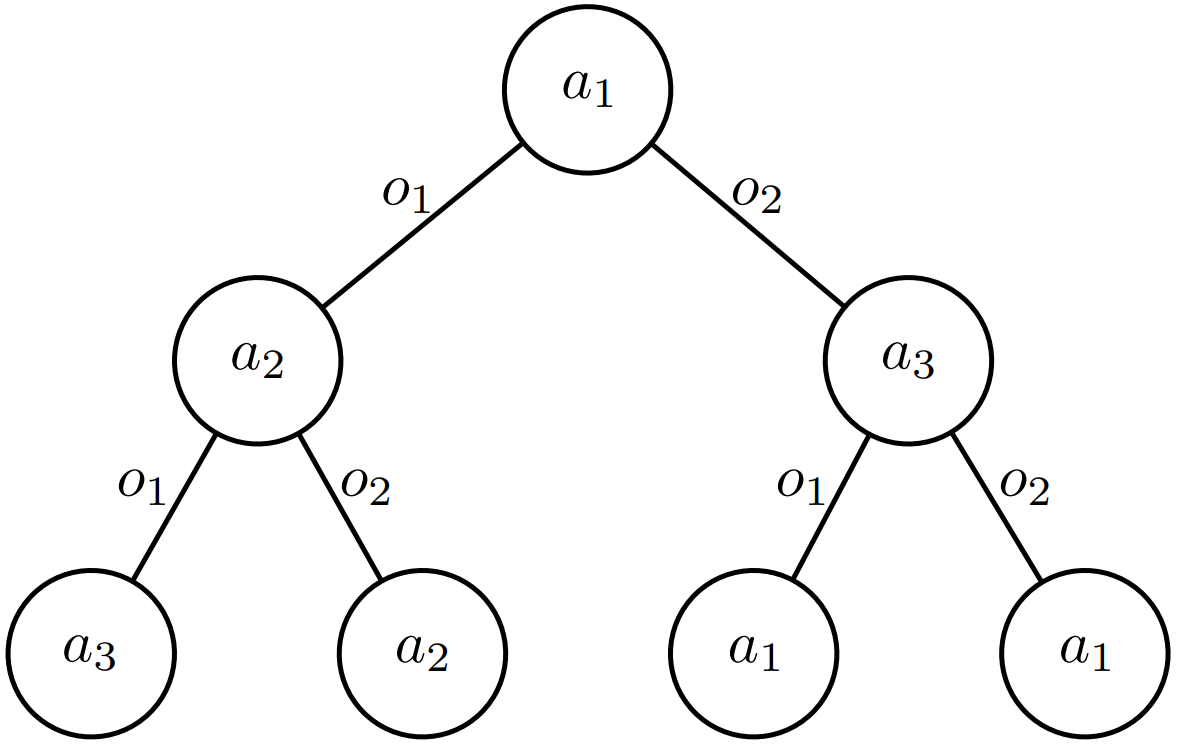
\includegraphics[width=\textwidth]{pt.png}
        \subcaption{Policy tree.}
    \end{subfigure} \hspace{6mm}
    \begin{subfigure}[b]{.12\textwidth}
        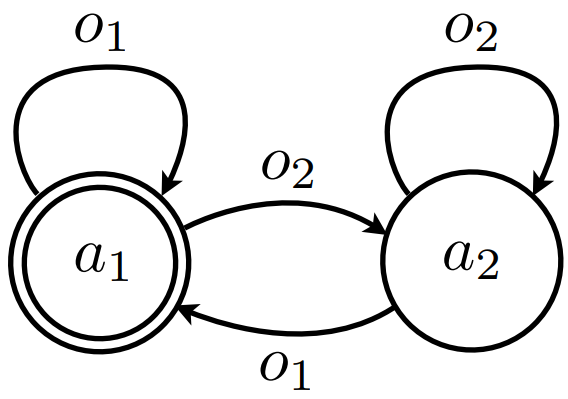
\includegraphics[width=\textwidth]{fsc.png}
        \subcaption{FSC.}
    \end{subfigure}
\vspace{-4mm}
\end{figure}

\subsection{Optimal Approaches}

\paragraph{Bottom-up} DP uses joint belief to find optimal solutions with policy pruning \cite{hansen2004dynamic}. 

\begin{equation}
    V^{t+1}(b^t) = \max_{a \in \mathcal{A}} \left\{ \sum_{s \in \mathcal{S}} b^t(s) 
\left[ R(s, a) + \sum_{o \in \mathcal{O}} \mathcal{P}(o \mid s, a) V^t(b^{t+1}) \right] \right\}.
\end{equation}

\begin{algorithm}[H]
\caption{DP Backup with Policy Pruning in Dec-POMDP}
\textbf{Input:} Depth-$t$ policy trees $Q_i^t$ and value vectors $V_i^t$ for each $i$
\begin{algorithmic}[1]
\STATE Perform exhaustive backups to get $Q_i^{t+1}$, and compute $V_i^{t+1}$ accordingly for each $i$
\REPEAT
    \STATE Find a policy tree $q_j \in Q_i^{t+1}$ that satisfies $\exists \ v_k \in \{V_i^{t+1} \setminus v_j\},b^{t+1} v_k \geq b^{t+1} v_j, \forall \ b^{t+1}$
    \STATE $Q_i^{t+1} \gets \{Q_i^{t+1} \setminus q_j\}$, and $V_i^{t+1} \gets \{V_i^{t+1} \setminus v_j\}$ accordingly
\UNTIL{no more pruning for all $i$}
\end{algorithmic}
\textbf{Output:} Depth-$t+1$ policy trees $Q_i^{t+1}$ and value vectors $V_i^{t+1}$ for each $i$
\end{algorithm}

\paragraph{Top-down} The policy tree can also be built using heuristic search like MAA* \cite{szer2005maa}.
\begin{algorithm}
\caption{MAA* Heuristic Search}
\textbf{Initialize:} Joint policy tree root $\Pi\gets\times_i \mathbb{A}_i$\\
\textbf{Input:} Depth-$t$ joint policy tree $\Pi$
\begin{algorithmic}[1]
    \STATE Select $a^*=\argmax_{a\in \Pi}F^\mathcal{H}(b^0, a)$ (heuristic and value)
    \STATE Expand $a^*$ to $a^\circledast$, and $\Pi \gets \{\Pi \cup  a^\circledast\}$
    \FOR {Each $a \in \Pi$}
    \IF {$F^\mathcal{H}(s^0, a^\circledast)\geqslant F^\mathcal{H}(s^0, a)$}
           \STATE $\Pi \gets \{\Pi \setminus a\}$
    \ENDIF
    \ENDFOR
    \IF {$a^*$ is fully expanded}
        \STATE $\Pi \gets \{\Pi \setminus a^*\}$
    \ENDIF
\end{algorithmic}
\textbf{Input:} Updated joint policy set $\Pi$.
\end{algorithm}

\subsection{Approximation Approaches}

The algorithms below improve scalability to larger problems over optimal methods, but do not possess any bounds on solution quality.

\paragraph{MBDP} Memory-bounded dynamic programming (MBDP) techniques mitigate the scalability problem of DP (which generates and evaluates all joint policy trees before pruning) by keeping a fixed number of policy trees for each agent at each step \cite{Seuken2007}. Several approaches have improved on MBDP by limiting \cite{Seukenimproved2007} or compressing \cite{Carlin2008} observations, replacing exhaustive backup with branch-and-bound search in the space of joint policy trees \cite{Dibangoye2009} as well as constraint optimization \cite{Kumar2010} and linear programming \cite{Wu2010} to increase the efficiency of selecting the best trees at each step.

\paragraph{JESP} The joint equilibrium search for policies (JESP) \cite{nair2003taming} uses alternating best response. Initial policies are generated for all agents, and then all but one is held fixed. The remaining agent can then calculate the best response (local optimum) to the fixed policies. The policy of this agent becomes fixed and the next agent calculates the best response. These best-response calculations to fixed other agent policies continue until no agent changes its policy.

\bibliography{ref}
\bibliographystyle{ref}

\clearpage
\appendix

\section{Complexity Classes} \label{appendix:complex}

Assuming $c$ and $k$ are constants, $\mathcal{C}$ is a complexity class, the table shows complexity terminologies.

\begin{table}[h!] \label{tab:complexitydefinition}
    \begin{tabular}{ll}
    \hline \hline
        P & the set of problems solvable in polynomial time, e.g., $O(n^k)$\\
        NP & the set of problems solvable nondeterministically in polynomial time \\
        EXP & the set of problems solvable in exponential time, e.g., $O(c^{n^k})$\\
        NEXP & the set of problems solvable nondeterministically in exponential time\\
        PSPACE & the set of problems solvable in polynomial space (P and NP $\subset$ PSPACE), e.g., $O(c^{n^k})$\\
        $\mathcal{C}$-hard & a problem that all problems in $\mathcal{C}$ are reducible to within  polynomial time\\
        $\mathcal{C}$-complete & a problem that is contained in $\mathcal{C}$ and $\mathcal{C}$-hard\\
    \hline \hline
    \end{tabular}
\end{table}

\end{document}
